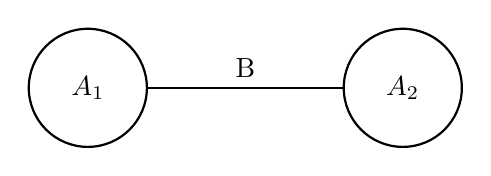
\begin{tikzpicture}[thick, scale=0.8]
  % Nodes
  \node[circle, draw, minimum size=1.5cm] (A1) at (0,0) {$A_1$};
  \node[circle, draw, minimum size=1.5cm] (A2) at (5,0) {$A_2$};
  
  % % Loops
  % \draw (A) circle (0.5) node[above right] {1};
  % \draw (B) circle (0.5) node[above left] {2};
  
  % Path
  \draw[-] (A1) -- (A2) node[midway, above] {B};
\end{tikzpicture}